\section{Geometria}

\questao{(OM$^3$SP 2026 - 2ª Fase) Tales de Mileto (c. 624 – 548 a.C.), foi um comerciante, matemático e astrônomo nascido na colônia jônica de Mileto (atual Turquia), é amplamente considerado por Aristóteles e pela tradição historiográfica como o primeiro filósofo do Ocidente e um dos Sete Sábios da Grécia Antiga. Uma proposição atribuída a ele é a Lei Angular de Tales que diz,} 

                \begin{Teorema}{Lei Angular de Tales}
                     Dado um triângulo de vértices $A$, $B$ e
                     $C$, de ângulos internos $\widehat A$, $\widehat B$ e $\widehat C$, a soma dos ângulos internos deste triângulo equivale a $180\text{°}$.
                \end{Teorema}
                \begin{figure}[H]
                    \centering
                    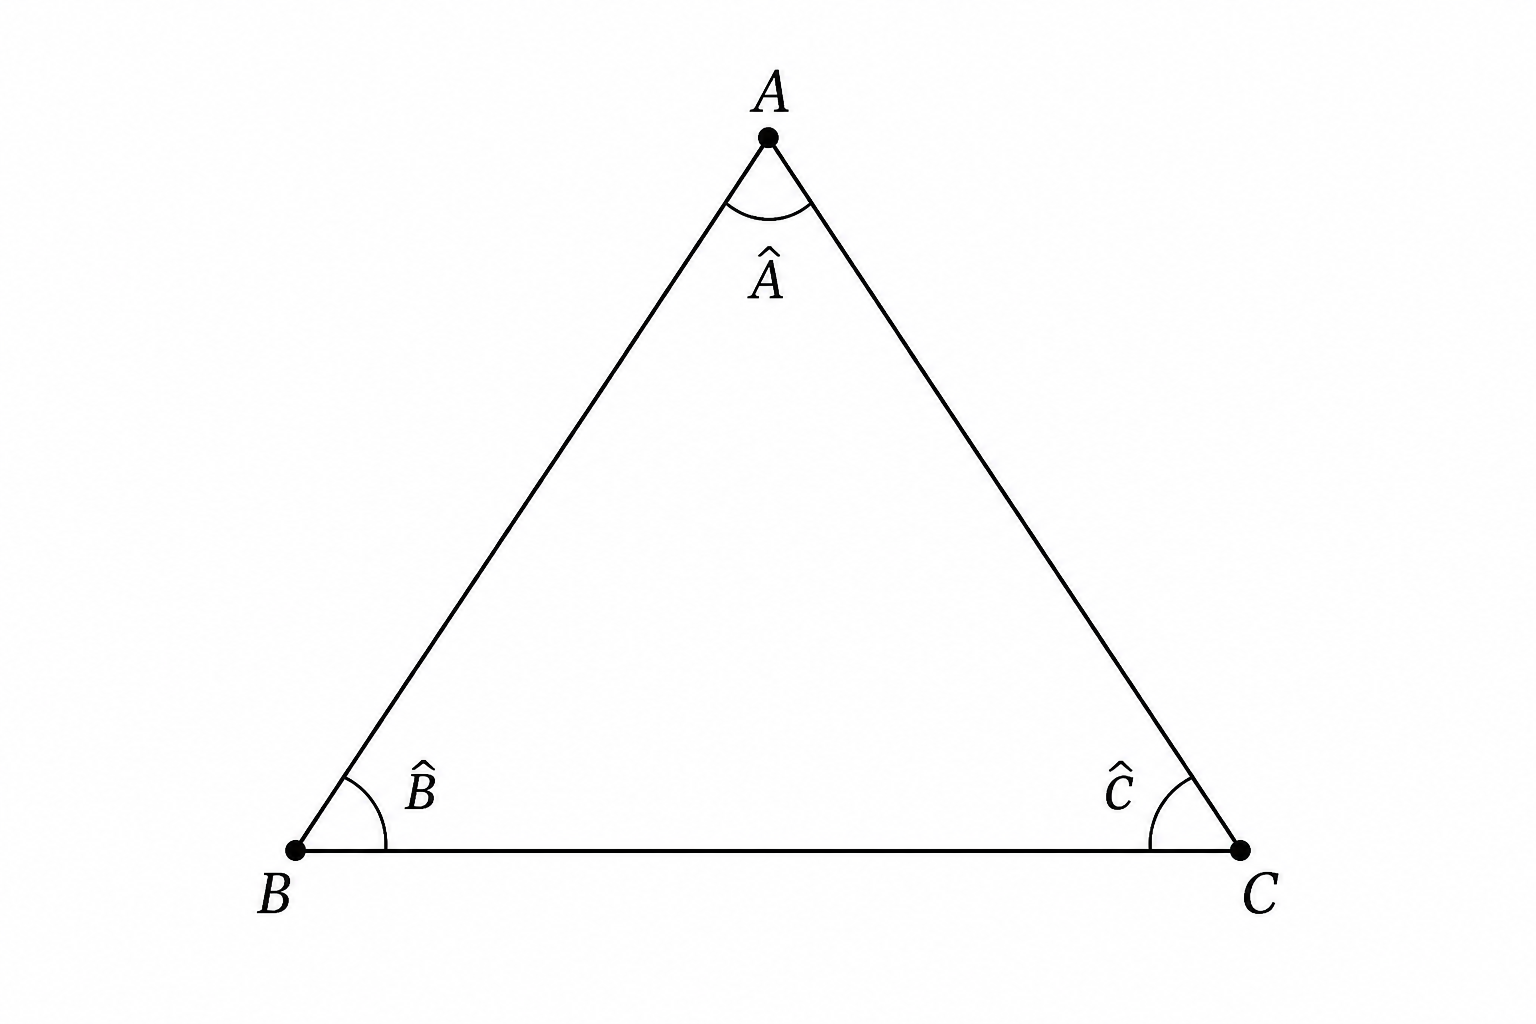
\includegraphics[width=0.45\linewidth]{figuras/7_ano/Max_a_Marque_também_os_vér.png}
                \end{figure}
           \begin{enumerate}[label=\alph*)]  
           \item Assumindo que o Teorema 1 é válido, qual será o valor do ângulo interno desconhecido de um triângulo, sabendo que os outros dois valem $25\text{°}$ e $120\text{°}$?
           
            \item Com base no que foi dito no Teorema 1, demostre que o que foi afirmado é possível.           
\item Em consequência ao item b, é possível determinar um teorema muito importante,
\begin{Teorema}{Teorema do Ângulo Externo}
     Dado um triângulo de vértices $A$, $B$ e $C$, de ângulos internos $\widehat A$, $\widehat B$ e $\widehat C$, o ângulo externo ao ângulo interno $\widehat C$ equivale a soma dos ângulos $\widehat A$ e $\widehat B$ .
\end{Teorema}
Com base no que foi dito no Teorema 2, demostre que o que foi afirmado é possível.
\end{enumerate}
% Caso a questão tenha mais de uma solução, alterar o valor da segunda chaves, que se refere ao valor para a quantidade de soluções que a questão terá.
% e insira o comando \solucao para uma nova resolução do item.

\begin{solucoes}{1}
    \solucao
\textbf{Item a)}

    Em primeiro lugar, não se deve fazer nada mais do que apenas utilizar o Teorema 1 proposto. Assim, assumindo que ele é válido e tendo dois ângulos determinados, no valor de $25\text{°}$ e $120\text{°}$,
    
\begin{equation*}
    \widehat A+ \widehat B+ \widehat C=180\text{°}
\end{equation*}
\begin{equation*}
    25\text{°}+120\text{°}+\widehat C=180\text{°}
\end{equation*}
\begin{equation*}
    145\text{°}+\widehat C=180\text{°}
\end{equation*}
\begin{equation*}
     \widehat C=180\text{°}-145\text{°}
\end{equation*}
\begin{equation*}
    \fbox{$\widehat C=35\text{°}$}
\end{equation*}

Logo, considerando que o Teorema 1 é válido, o valor do ângulo interno desconhecido será $35\text{°}$.
\end{solucoes}

% Caso a questão tenha mais de uma solução, alterar o valor da segunda chaves, que se refere ao valor para a quantidade de soluções que a questão terá.
% e insira o comando \solucao para uma nova resolução do item.
\begin{solucoes}{1}

\solucao

\textbf{Item b)}

Após mostrar a usualidade do Teorema 1 no \textbf{item a)}, uma pergunta deve surgir: Será que este Teorema é sempre válido? Dentro da geometria euclidiana, ele será sempre válido, todavia é preciso que se prove esta verdade. Sendo assim, considere um triângulo de vértices  $A, B \ \text{e} \ C$, se traçarmos uma reta tangente ao vértice $A$ e prolongarmos as retas que passam pelos vértices $A, B \ \text{e} \ C$, teremos

\begin{figure}[H]
    \centering
    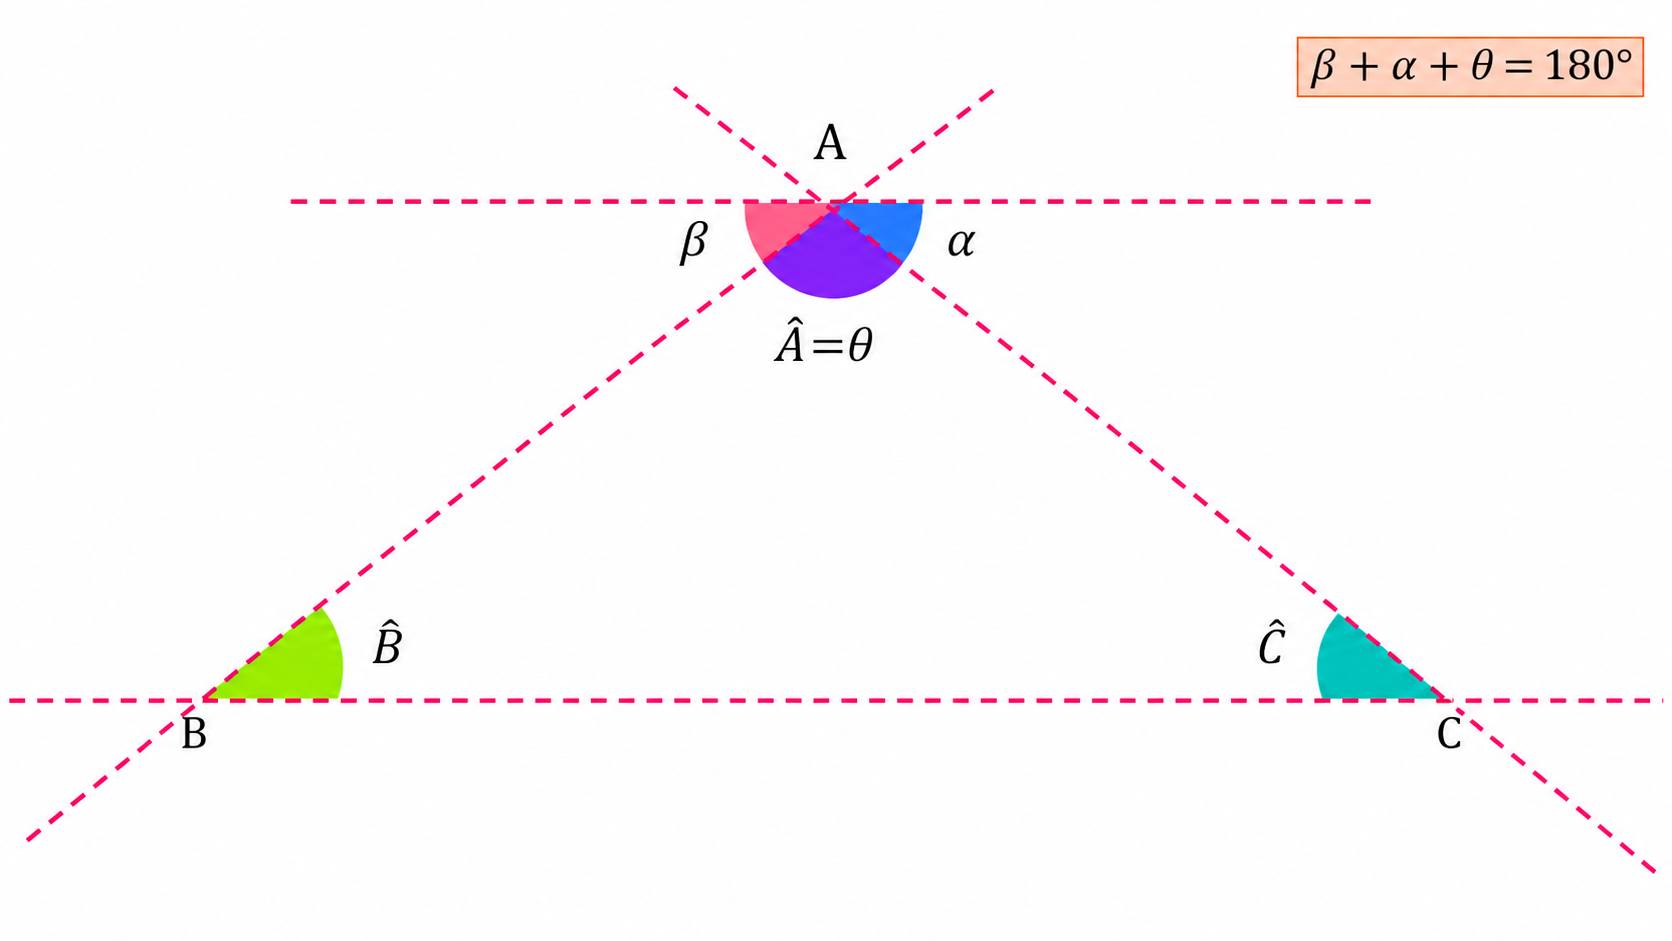
\includegraphics[width=0.7\linewidth]{figuras/7_ano/Max_a_gere_esta_imagem_em_.png}
\end{figure}

Perceba, no triângulo acima, que os ângulos $\alpha$, $\beta$ e $\widehat A \equiv \theta$ somados totalizam $180\text{°}$. Se observarmos bem, temos que o ângulo $\beta$ é correspondente ao ângulo que está oposto pelo vértice ao ângulo $\widehat B$ e o ângulo $\alpha$ é correspondente ao ângulo que está oposto pelo vértice ao ângulo $\widehat C$, como a imagem a seguir nos mostra,
\begin{figure}[H]
    \centering
    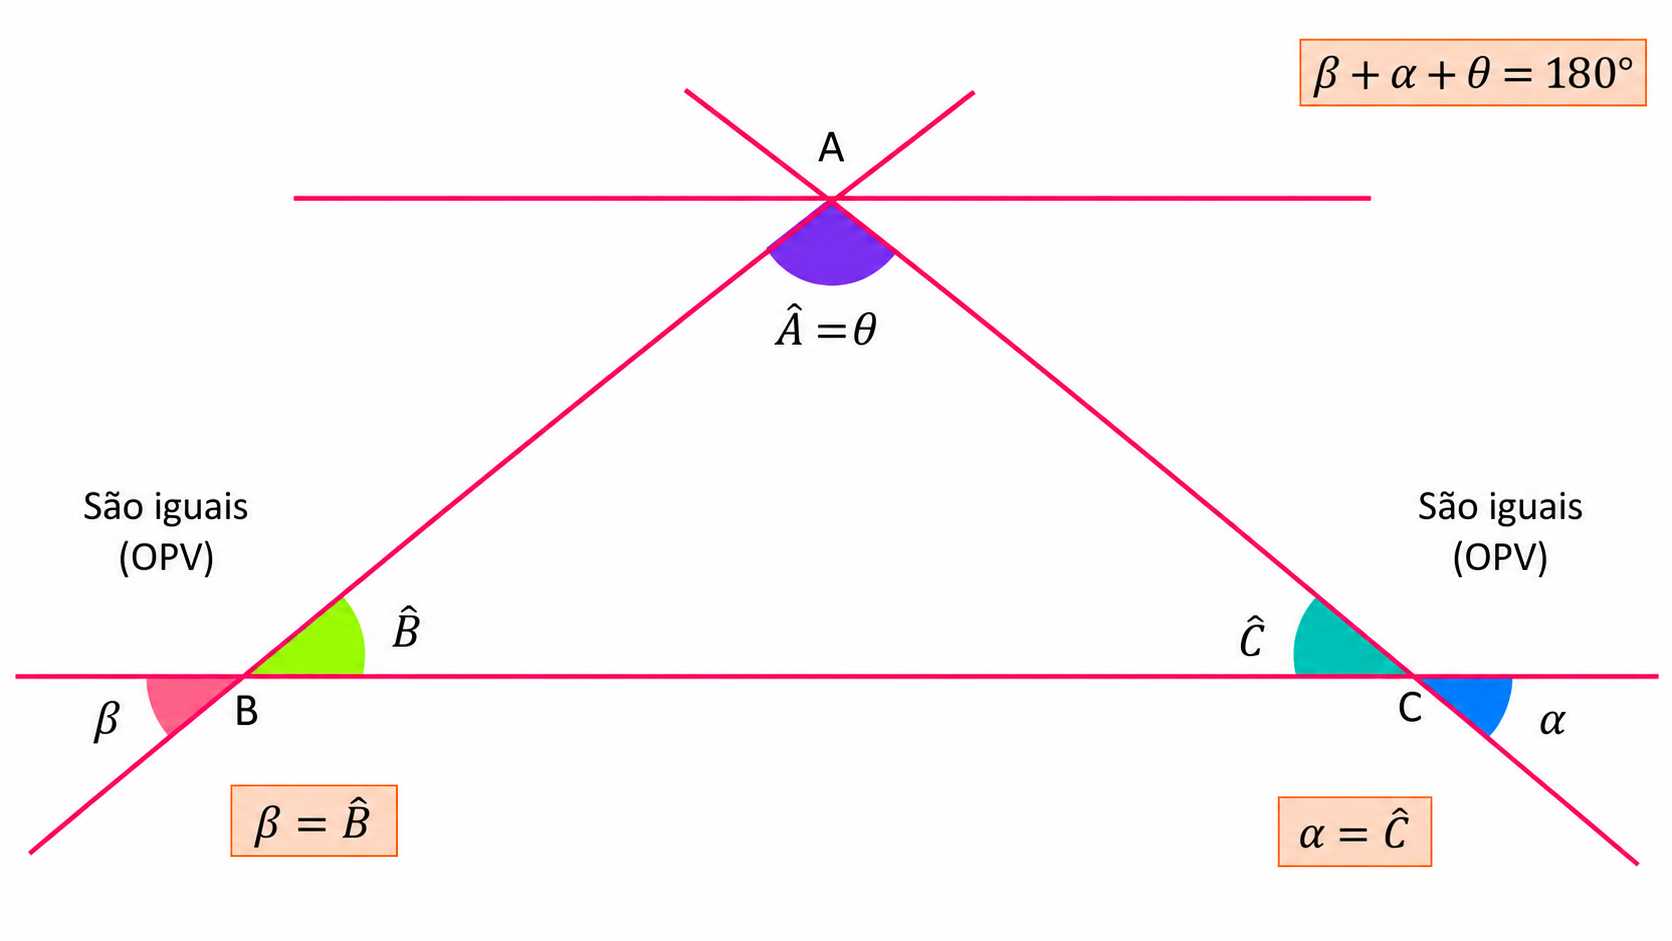
\includegraphics[width=0.7\linewidth]{figuras/7_ano/Max_a_gere_esta_imagem_em_ (1).png}
    \label{fig:placeholder}
\end{figure}
    Por definição, dois ângulos que são opostos pelo vértice são congruentes. Logo, $\beta \equiv \widehat B$ e $\alpha \equiv \widehat C$. Com isso, chegamos à conclusão do item b, pois 
    \begin{equation*}
        \alpha+\beta+\theta=180^°
    \end{equation*}
e como $\alpha \equiv \widehat C$, $\widehat A \equiv \theta$ e $\beta \equiv \widehat B$, concluímos que
    \begin{equation*}
        \widehat A+\widehat B+\widehat C=180^°
    \end{equation*} 

\solucao

\textbf{Item c)} 

Após mostrar a lei angular de Tales, o Teorema do ângulo Externo se torna quase que uma consequência. Observe a figura a seguir,
\begin{figure}[H]
    \centering
    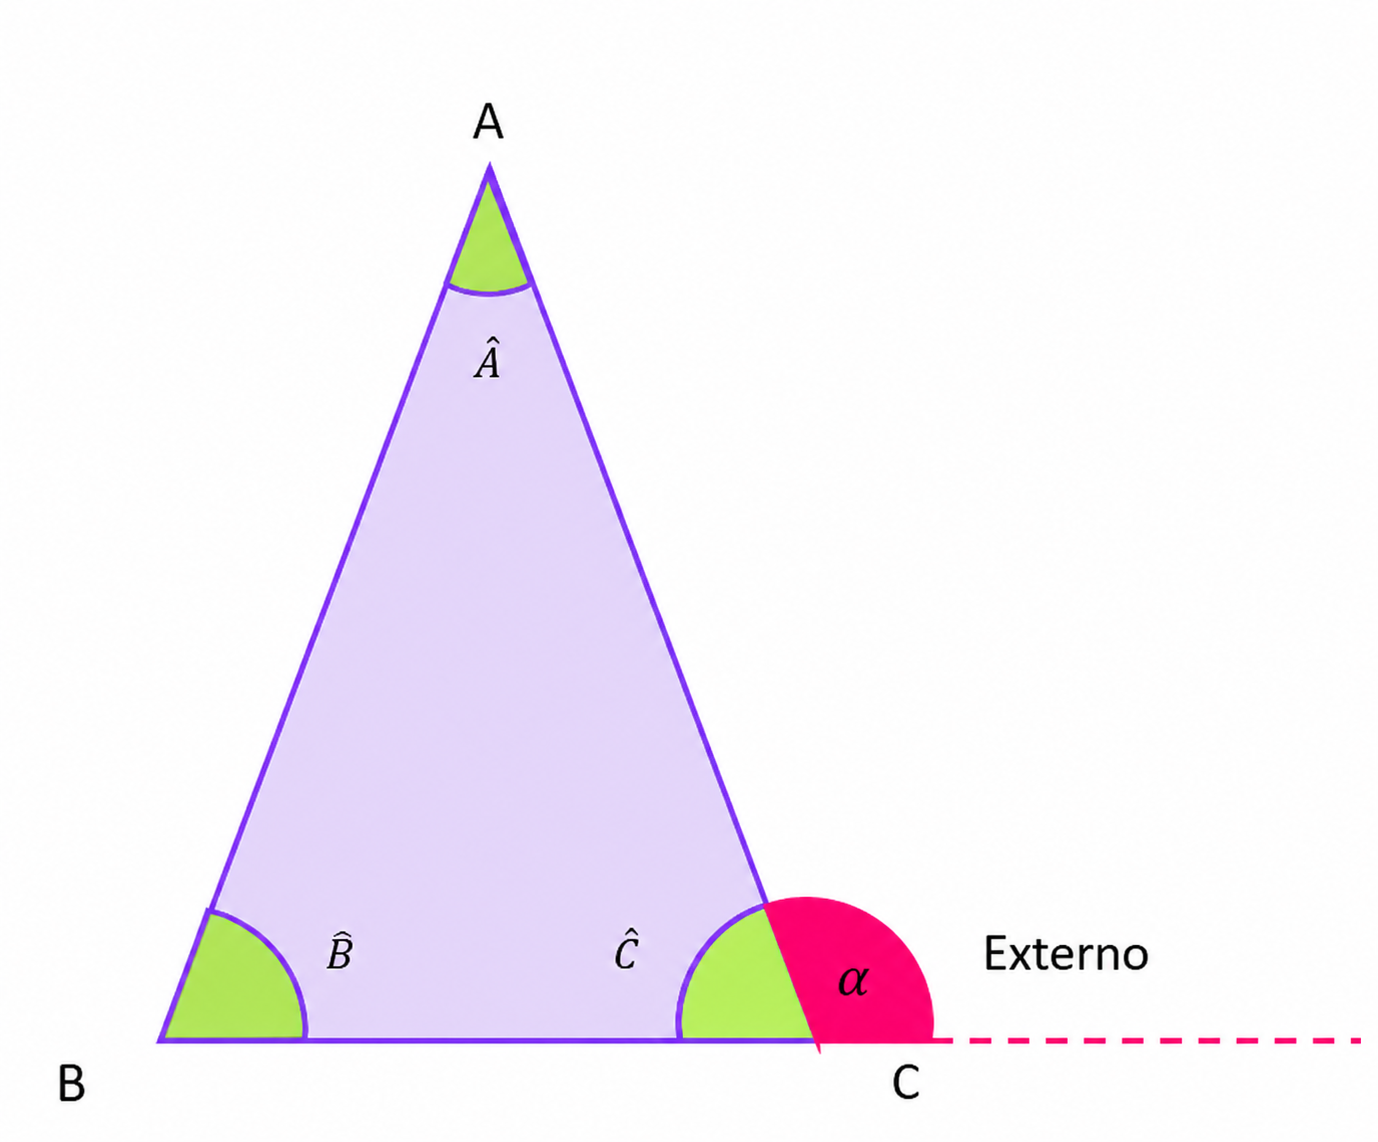
\includegraphics[width=0.45\linewidth]{figuras/7_ano/Max_a_não_mude_nada_da_fot.png}
    \label{fig:placeholder}
\end{figure}
Duas coisas devem saltar aos nossos olhos. Em primeiro lugar, pelo item b) sabemos que $ \widehat A+\widehat B+\widehat C=180^\textit{°}$. Em segundo, e último lugar, sabemos que $\widehat C+\alpha=180\textit{°}$, pois os dois são ângulos suplementares. Após essas duas definições só nos resta utilizarmos as ferramentas aritméticas para resolver este enigma e assim,
\begin{equation*}
  \begin{cases}
    \widehat A+\widehat B+\widehat C=180^° \\
    \widehat C+\alpha=180\textit{°}
  \end{cases}
\end{equation*}
Se pegarmos a primeira equação e subtrai-la pela segunda teremos que

\begin{equation*}
    \widehat A+\widehat B-\alpha=0 
\end{equation*}
\begin{equation*}
        \widehat A+\widehat B=\alpha
\end{equation*}
Logo, o ângulo externo ao ângulo $\widehat C$ equivale a soma dos ângulos internos $\widehat A \ e \ \widehat B$.
\end{solucoes}

\questao{(OM$^3$SP 2026 - 1$^\circ$ fase) Um jogo de Tangram foi montado a partir de sete peças recortadas de um quadriculado, no qual cada quadradinho possui lado de 1 cm, conforme ilustrado na figura a seguir.}

        \begin{center}
            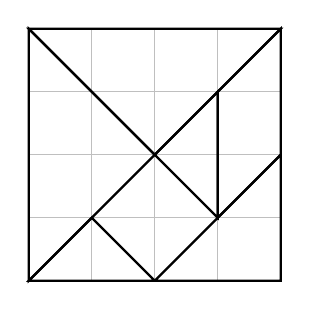
\begin{tikzpicture}[scale=.8]
                \draw[step=1cm, very thin, gray!50](0,0) grid (4,4);

                \draw[thick](0,0)--(2,2)--(0,4) -- cycle;
                \draw[thick](2,2)--(4,4)--(0,4)--cycle;
                \draw[thick](0,0)--(1,1)--(2,0)-- cycle;
                \draw[thick](2,2)--(3,1)--(3,3)-- cycle;
                \draw[thick](2,0)--(4,0)--(4,2)-- cycle;
                \draw[thick](3,1)--(4,2)--(4,4)--(3,3)--cycle;
                
            \end{tikzpicture}
        \end{center}

         A figura a seguir foi montada com 5 dessas peças sem sobreposição. Qual é a área dessa figura?

        \begin{figure}[H]
            \begin{minipage}{.34\linewidth}
                \begin{enumerate}[label=\alph*)]
                    \item 10 $cm^2$
                    \item 12 $cm^2$
                    \item 14 $cm^2$
                    \item 16 $cm^2$
                \end{enumerate}
            \end{minipage}
            \begin{minipage}{.65\linewidth}
                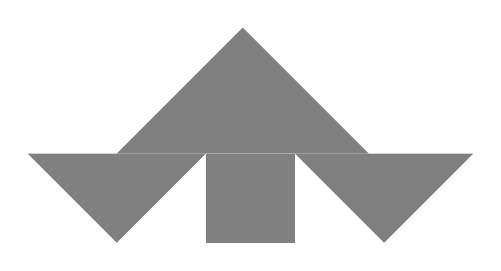
\begin{tikzpicture}[scale=.8]
                    \fill[color=black!50, thick, rotate around={-45:(1,1)}](0,0)--(2,0)--(1,1)--cycle;
                    \fill[color=black!50, thick, rotate around={45:(1,1)}](0,0)--(2,0)--(1,1)--cycle;
                    \fill[color=black!50, thick](2.4142,1)rectangle(3.8284,-.4142);
                    \fill[color=black!50, thick](1,1)--(5,1)--(3,3)--cycle;
                    \fill[color=black!50, thick](3.8284,1)--(5.2426,-.4142)--(6.6568,1)--cycle;
                \end{tikzpicture}
            \end{minipage}
        \end{figure}

\begin{solucoes}{1}
    \solucao
    
Sabendo que a área do tangram completa é de 16cm$^2$ e que para criar essa figura, foi utilizado 5 peças do tangram, podemos descobrir quais foram essas peças, pelo formato do triangulo maior, podemos concluir que foi utilizado um triangulo grande, dois triangulos pequenos, um triangulo medio e um quadrado.

Dessa forma, utilizando a figura do tangram completo de referencia, podemos calcular a area de cada uma dessas peças utilizadas na construção da figura.

Para o triângulo maior, temos que sua área é:

$\begin{WithArrows}
    A_{T. maior}=&\dfrac{4\times2}{2} \\
    A_{T. maior}=&4\, cm^2
\end{WithArrows}$

Para o triângulo médio, temos que sua área pega um quadrado de 1cm$^2$ e duas metades de um quadrado completo, ou seja, 2 $\times\,\dfrac{1}{2}cm^2$, assim, a área do triangulo médio é de $2cm^2$

Para os dois triângulo menores, temos que sua área é duas metades de um quadrado completo, assim, 2 $\times\,\dfrac{2 \times 1}{2}cm^2$, logo, a soma das áreas dos dois triângulos menores é igual a $2cm^2$

E por fim, temos a área do quadrado, observa-se que o quadrado é formado por 4 metades de quadrados, sendo assim, sua área é 4 $\times\, \dfrac{1}{2}cm^2$, ou seja, 2$cm^2$

então, a área formada por todas essas partes é a soma dessas áreas, deste modo, temos:

A$_{figura}$ = A$_{T. maior}$ + A$_{T. medio}$ + A$_{T. pequeno}$ + A$_{quadrado}$ = 4$cm^2$ + 2$cm^2$ + 2$cm^2$ + 2$cm^2$ 

A$_{figura}$ = 10$cm^2$

\textbf{Alternativa A}
\end{solucoes}

\questao{(OM$^3$SP 2026 - 2ª Fase) Na aula de Geografia, a professora Patrícia trouxe dois mapas que tinham o formato superficial de duas figuras geométricas distintas, um quadrado e um retângulo. Os alunos perceberam que as superfícies tinham algumas características comuns aos dois. Qual a característica comum as duas figuras quanto aos seus ângulos internos ($a_i$)?}
        \begin{multicols}{4}
            \begin{enumerate}[label=\alph*)]
                \item $a_i=90^\circ$
                \item $a_i=60^\circ$
                \item $a_i=45^\circ$
                \item $a_i=30^\circ$
            \end{enumerate}
        \end{multicols}

\begin{solucoes}{1}
    \solucao
    Ao comparar-se dois mapas, tem-se que as figuras que os dispõem são um quadrado e um retângulo. Essas figuras possuem muitas semelhanças e quanto aos seus ângulos internos, tem-se uma semelhança notável: todos os ângulos internos de um retângulo e um quadrado são ângulos retos. Sendo assim, $a_i=90^\circ$.\\
    \textbf{ALTERNATIVA A}
\end{solucoes}


